\RequirePackage{currfile}
\documentclass[12pt]{beamer}
\usepackage[utf8]{inputenc}
\usepackage[spanish]{babel}
\usepackage{standalone}
\usepackage{color}
\usepackage{siunitx}
\usepackage{hyperref}
%\hypersetup{colorlinks,linkcolor=,urlcolor=blue}
%\hypersetup{colorlinks,urlcolor=blue}
\usepackage{xcolor,soul}
\usepackage{etoolbox}
\usepackage{amsmath}
\usepackage{amsthm}
\usepackage{physics}
\usepackage{multicol}
\usepackage{bookmark}
\usepackage{longtable}
\usepackage{listings}
\lstset{
basicstyle=\ttfamily,
columns=fullflexible,
breaklines=true
}
\usepackage{graphicx}
\usepackage{tikz}
\usetikzlibrary{matrix, backgrounds, decorations,shapes, arrows.meta}
\usepackage[autostyle,spanish=mexican]{csquotes}
\usepackage[os=win]{menukeys}
\usepackage{pifont}
\usepackage{pbox}
\usepackage{caption}
\captionsetup{font=scriptsize,labelfont=scriptsize}
\usepackage{dcolumn}
\newcolumntype{L}{D{.}{.}{2,5}}

\definecolor{ao}{rgb}{0.0, 0.5, 0.0}
\definecolor{bisque}{rgb}{1.0, 0.89, 0.77}
\definecolor{amber}{rgb}{1.0, 0.75, 0.0}
\definecolor{armygreen}{rgb}{0.29, 0.33, 0.13}
\definecolor{alizarin}{rgb}{0.82, 0.1, 0.26}
\definecolor{cadetblue}{rgb}{0.37, 0.62, 0.63}
\definecolor{deepblue}{rgb}{0,0,0.5}
\definecolor{brown}{rgb}{0.59, 0.29, 0.0}
\definecolor{OliveGreen}{rgb}{0,0.25,0}

\definecolor{Code}{rgb}{0,0,0}
\definecolor{Keywords}{rgb}{255,0,0}
\definecolor{Strings}{rgb}{255,0,255}
\definecolor{Comments}{rgb}{0,0,255}
\definecolor{Numbers}{rgb}{255,128,0}


\newcommand*{\TitleParbox}[1]{\parbox[c]{1.75cm}{\raggedright #1}}%

%\usepackage[sfdefault]{roboto}  %% Option 'sfdefault' only if the base font of the document is to be sans serif

\renewcommand{\arraystretch}{1.5}
\renewcommand{\rmdefault}{cmr}% cmr = Computer Modern Roman
\usefonttheme[onlymath]{serif}

\newcommand{\python}{\texttt{python}}
\newcommand{\textoazul}[1]{\textcolor{blue}{#1}}
\newcommand{\azulfuerte}[1]{\textcolor{blue}{\textbf{#1}}}
\newcommand{\funcionazul}[1]{\textcolor{blue}{\textbf{\texttt{#1}}}}

\newcounter{saveenumi}
\newcommand{\seti}{\setcounter{saveenumi}{\value{enumi}}}
\newcommand{\conti}{\setcounter{enumi}{\value{saveenumi}}}

\linespread{1.5}
\beamertemplatenavigationsymbolsempty
\usefonttheme{professionalfonts}
%\usefonttheme{serif}
\DeclareGraphicsExtensions{.pdf,.png,.jpg}
\renewcommand {\arraystretch}{1.25}
\mode<presentation>
{
  \usetheme{Warsaw}
  \setbeamertemplate{headline}{}
  %\useoutertheme{infolines}
  \useoutertheme{default}
  \setbeamercovered{invisible}
  % or whatever (possibly just delete it)
  \setbeamertemplate{section in toc}[sections numbered]
  \setbeamertemplate{subsection in toc}[subsections numbered]
  \setbeamertemplate{subsection in toc}{\leavevmode\leftskip=3.2em\rlap{\hskip-2em\inserttocsectionnumber.\inserttocsubsectionnumber}\inserttocsubsection\par}
  \setbeamercolor{section in toc}{fg=blue}
  \setbeamercolor{subsection in toc}{fg=blue}
  \setbeamercolor{frametitle}{fg=yellow}

  \setbeamertemplate{footline} 
{
  \leavevmode%
  \hbox{%
  \begin{beamercolorbox}[wd=.333333\paperwidth,ht=2.25ex,dp=1ex,center]{author in head/foot}%
    \usebeamerfont{author in head/foot}\insertsection
  \end{beamercolorbox}%
  \begin{beamercolorbox}[wd=.333333\paperwidth,ht=2.25ex,dp=1ex,center]{title in head/foot}%
    \usebeamerfont{title in head/foot}\textcolor{yellow}{\insertsubsection}
  \end{beamercolorbox}%
  \begin{beamercolorbox}[wd=.333333\paperwidth,ht=2.25ex,dp=1ex,right]{date in head/foot}%
    \usebeamerfont{date in head/foot}\insertshortdate{}\hspace*{2em}
    \insertframenumber{} / \inserttotalframenumber\hspace*{2ex} 
  \end{beamercolorbox}}%
  \vskip0pt%
}
}
\makeatother

\makeatletter
\patchcmd{\beamer@sectionintoc}
  {\vfill}
  {\vskip\itemsep}
  {}
  {}
\makeatother

% \makeatletter
% \patchcmd{\hyper@link@}
%   {{\Hy@tempb}{#4}}
%   {{\Hy@tempb}{\ul{#4}}}
%   {}{}
% \makeatother

\DeclareCaptionFont{white}{\color{white}}
\DeclareCaptionFormat{listing}{\colorbox{gray}{\parbox{0.99\textwidth}{#1#2#3}}}
\captionsetup[lstlisting]{format=listing,labelfont=white,textfont=white}
\renewcommand{\lstlistingname}{Código}

\lstdefinestyle{codigopython}{%
  language=Python,                % choose the language of the code
  %basicstyle=\footnotesize\small,       % the size of the fonts that are used for the code
  numbers=left,                   % where to put the line-numbers
  numberstyle=\scriptsize,      % the size of the fonts that are used for the line-numbers
  stepnumber=1,                   % the step between two line-numbers. If it is 1 each line will be numbered
  numbersep=5pt,                  % how far the line-numbers are from the code
  backgroundcolor=\color{white},  % choose the background color. You must add \usepackage{color}
  showspaces=false,               % show spaces adding particular underscores
  showstringspaces=false,         % underline spaces within strings
  showtabs=false,                 % show tabs within strings adding particular underscores
  frame=single,   		% adds a frame around the code
  tabsize=2,  		% sets default tabsize to 2 spaces
  captionpos=t,   		% sets the caption-position to bottom
  breaklines=true,    	% sets automatic line breaking
  breakatwhitespace=false,    % sets if automatic breaks should only happen at whitespace
  escapeinside={\#},  % if you want to add a comment within your code
  stringstyle =\color{OliveGreen},
  texcl = true,
  %otherkeywords={{as}},             % Add keywords here
  keywordstyle = \color{blue},
  commentstyle = \color{black},
  identifierstyle = \color{black},
  % literate=%
  %         {á}{{\'a}}1
  %         {é}{{\'e}}1
  %         {í}{{\'i}}1
  %         {ó}{{\'o}}1
  %         {ú}{{\'u}}1
  %
  %keywordstyle=\ttb\color{deepblue}
  %fancyvrb = true,
literate={0}{{\textcolor{red}{0}}}{1}%
            {1}{{\textcolor{red}{1}}}{1}%
            {2}{{\textcolor{red}{2}}}{1}%
            {3}{{\textcolor{red}{3}}}{1}%
            {4}{{\textcolor{red}{4}}}{1}%
            {5}{{\textcolor{red}{5}}}{1}%
            {6}{{\textcolor{red}{6}}}{1}%
            {7}{{\textcolor{red}{7}}}{1}%
            {8}{{\textcolor{red}{8}}}{1}%
            {9}{{\textcolor{red}{9}}}{1}%
            {.0}{{\textcolor{red}{.0}}}{2}% Following is to ensure that only periods
            {.1}{{\textcolor{red}{.1}}}{2}% followed by a digit are changed.
            {.2}{{\textcolor{red}{.2}}}{2}%
            {.3}{{\textcolor{red}{.3}}}{2}%
            {.4}{{\textcolor{red}{.4}}}{2}%
            {.5}{{\textcolor{red}{.5}}}{2}%
            {.6}{{\textcolor{red}{.6}}}{2}%
            {.7}{{\textcolor{red}{.7}}}{2}%
            {.8}{{\textcolor{red}{.8}}}{2}%
            {.9}{{\textcolor{red}{.9}}}{2}%
            {\ }{{ }}{1}% handle the space
        ,%
        %mathescape=true
        %escapeinside={*@}
        escapeinside={A_}{_B}
}

\title{Tema 0 - Funciones y Graficación con \python}
\author[]{M. en C. Gustavo Contreras Mayén \\ M. en C. Abraham Lima Buendía}
\institute{Facultad de Ciencias - UNAM}
\titlegraphic{
\includegraphics[width=2cm]{escudo-facultad-ciencias}\hspace*{4.75cm}~%
   
\includegraphics[width=2cm]{escudo-unam}
}
\date{\today}
\begin{document}
\maketitle
\section*{Contenido}
\frame[allowframebreaks]{\tableofcontents[currentsection, hideallsubsections]}
\fontsize{14}{14}\selectfont
\spanishdecimal{.}
\section{Funciones}
\frame[allowframebreaks]{\tableofcontents[currentsection, hideothersubsections]}
\subsection{Estructura de una función}
\begin{frame}
\frametitle{Las funciones en \python}
Con lo que hemos revisado sobre \python, tenemos elementos para iniciar la solución de problemas.
\\
\bigskip
Si agrupamos de manera particular un conjunto de instrucciones, entonces estaremos usando las llamadas \emph{funciones}.
\end{frame}
\begin{frame}[fragile]
\frametitle{Estructura de una función}
La palabra reservada \azulfuerte{def} se usa para definir funciones. 
\\
\bigskip
 Debe seguirle el nombre de la función (identificador), así como una lista de argumentos entre paréntesis, puede ocurrir que haya funciones que no ocupen argumentos.
 \\
\bigskip
Las sentencias que forman el cuerpo de la función empiezan en la línea siguiente, y deben estar con sangría.
\end{frame}
\begin{frame}[fragile]
\frametitle{Estructura de una función}
La estructura de una función en \python{} es la siguiente:
\fontsize{12}{12}\selectfont
\begin{lstlisting}
def nombre_funcion(parametro1, parametro2, ...):
    conjunto de instrucciones
    return valores_devueltos
\end{lstlisting}
donde \texttt{parametro1,} \texttt{parametro2} son los parámetros. Un parámetro puede ser cualquier objeto de \python, incluyendo una función.
\end{frame}
\begin{frame}
\frametitle{Estructura de una función}
Los parámetros pueden darse por defecto, por lo que en la función son opcionales. 
\\
\bigskip
Si no se utiliza la instrucción \azulfuerte{return}, la función devuelve un objeto de tipo \azulfuerte{None}
\end{frame}
\begin{frame}[fragile]
\frametitle{Ejemplo de una función}
\begin{lstlisting}[style=codigopython]
def cuadrados(entrada):
    for i in range(len(entrada)):
        entrada[i] = entrada[i]**2
    return entrada

a = [1, 2, 3, 4]
respuesta = cuadrados(a)
print(respuesta)
\end{lstlisting}
\end{frame}
\begin{frame}
\frametitle{Cálculo de la serie de Fibonacci}
La sucesión fue descrita por Fibonacci como la solución a un problema de la cría de conejos: 
\\
\bigskip
\enquote{Cierto hombre tenía una pareja de conejos juntos en un lugar cerrado y uno desea saber cuántos son creados a partir de este par en un año, cuando es su naturaleza parir otro par en un simple mes, y en el segundo mes los nacidos parir también}
\\
\bigskip
\pause
\textcolor{red}{cómo le hacemos para calcular cuántos conejos hay?}
\end{frame}
\begin{frame}[fragile]
\frametitle{Propuesta de código}
\begin{lstlisting}[style=codigopython]
def fib(n):
    a, b = 0, 1
    while b < n:
        print (b)
        a, b = b, a + b
    
    return b

fib(2000)
\end{lstlisting}
\end{frame}
\begin{frame}[fragile]
\frametitle{Segunda propuesta de código}
\begin{lstlisting}[style=codigopython]
def fibA_2_B(n):
    resultado = []
    a, b = 0, 1
    while a < n:
        resultado.append(a)
        a, b = b, a + b
    return resultado

fibo100 = fib2(100)
print(fibo100)
\end{lstlisting}
\end{frame}
\subsection{Paso de argumentos}
\begin{frame}[fragile]
\frametitle{Paso de argumentos}
Para que una función sea en verdad útil (y reutilizable), es necesario que podamos pasarle datos a modo de \emph{entradas}. 
\\
\bigskip
Los nombres de las entradas (o argumentos) que requiere una función se declaran a continuación del nombre en \azulfuerte{def} (siempre entre paréntesis)
\end{frame}
\begin{frame}[fragile]
\frametitle{Ejemplo de función con argumentos}
\begin{lstlisting}
def FuncionSuma (x, y):
    return x + y

print(FuncionSuma(5, 3))
print(FuncionSuma(7, 42.0))
print(FuncionSuma(" hola ", " mundo "))
\end{lstlisting}
\end{frame}
\begin{frame}[fragile]
\frametitle{Ejemplo de función con argumentos}
\textbf{Notas:} 
\begin{itemize}[<+->]
\item Nunca se mencionan los tipos de datos para $x$ e $y$, ni el tipo de datos que devuelve FuncionSuma.
\item Los argumentos y el valor devuelto son, tal como las variables, simples etiquetas a zonas de memoria.
\end{itemize}  
\end{frame}
\subsection{Paso de argumento con nombre}
\begin{frame}
\frametitle{Paso de argumentos con nombre}
Si la función que definimos tiene muchos argumentos, es fácil olvidar el orden en que fueron declarados.
\\
\medskip
Como un argumento no lleva asociado un tipo, \python{} no tiene manera de saber que los argumentos están cambiados.
\end{frame}
\begin{frame}
\frametitle{Paso de argumentos con nombre}
Para evitar este tipo de errores, hay una manera de llamar a una función pasando los argumentos en cualquier orden arbitrario: se pasan usando el nombre usado en la declaración.
\end{frame}
\begin{frame}[fragile]
\frametitle{Ejemplo de paso de argumentos con nombre}
\begin{lstlisting}[style=codigopython]
def Prueba (a, b, c):
    print("a = {}, b = {}, c = {}".format(a, b, c))



Prueba (1, 2, 3)
Prueba (b = 3, a = 2, c = 1)
\end{lstlisting}
\end{frame}
\subsection{Argumentos con valores por omisión}
\begin{frame}[allowframebreaks, fragile]
\frametitle{Argumentos con valores por omisión}
Para hacer que algunos argumentos sean opcionales, se les da valores por omisión en el momento de declararlos:
\begin{lstlisting}[style=codigopython]
from math import sqrt

#el argumento v es necesario
def Gamma(v, c=3.0e+8):
    return sqrt(1.0-(v/c)A_**_B2)


#se modifica el valor de c
print(Gamma(0.1, 1.0))

#solo se pasa el valor de v
print(Gamma(1.e+7))
\end{lstlisting}
\end{frame}
\subsection{Devolviendo varios valores en una función}
\begin{frame}[fragile]
\frametitle{Devolviendo varios valores en una función}
Para hacer que una función devuelva más de un valor, lo que hacemos es definir argumentos de entrada y argumentos de salida.
\\
\bigskip
Veremos la manera en que se deben de ocupar los valores de salida, una vez que se cumple la función.
\end{frame}
\begin{frame}[fragile]
\frametitle{Devolviendo varios valores en una función}
Para devolver múltiples valores en \python, lo usual es devolver los valores \enquote{empaquetados} en una tupla:
\end{frame}
\begin{frame}[allowframebreaks,fragile]
\frametitle{Regresando varios valores en una función}
\begin{lstlisting}[style=codigopython]
from math import atanA_2_B, sqrt

def ModuloArgumento(x, y):
    norma = sqrt(xA_**_B2 + yA_**_B2)
    argumento = atanA_2_B(y, x)
    return (norma, argumento)


n, a = ModuloArgumento(3.0, 4.0)
print("El modulo es: ", n)
print("El argumento es: ", a)
\end{lstlisting}
\end{frame}
\subsection{Número variable de argumentos}
\begin{frame}[fragile]
\frametitle{Número variable de argumentos}
¿Cómo le hacemos para que una función acepte un número no prefijado de argumentos?
\\
\medskip
Es posible pasar una lista o tupla, pero \python{} ofrece una mejor solución:
\end{frame}
\begin{frame}[fragile, allowframebreaks]
\frametitle{Número variable de argumentos}
\begin{lstlisting}[style=codigopython]
from math import atan, atanA_2_B

#args es una tupla de argumentos
def atanVariable(*args):
    if len(args) == 1:
        return atan(args[0])
    else :
        return atanA_2_B(args[0], args[1])


print (atanVariable(0.2)) # 0.19739
print (atanVariable(2.0,10.0)) # 0.19739
print (atanVariable(-2.0,-10.0)) # -2.94419
\end{lstlisting}
\end{frame}
\subsection{Funciones lambda}
\begin{frame}
\frametitle{Funciones lambda}
\python{} admite una interesante sintaxis que permite definir funciones mínimas, de una línea sobre la marcha. 
\\
\bigskip
Se trata de las denominadas funciones \azulfuerte{lambda}, que pueden utilizarse en cualquier lugar donde se necesite una función.
\end{frame}
\begin{frame}[fragile, allowframebreaks]
\frametitle{Funciones lambda}
\begin{lstlisting}[style=codigopython]

#primera forma de una funcion lambda

numero = float(input("Introduce un numero real"))

g = lambda x: x*2
print(g(numero))

#segunda forma de escribir una funcion lambda

print((lambda x: x*2)(numero)) 
\end{lstlisting}
\end{frame}
\begin{frame}
\frametitle{Funciones lambda}
Nótese que: la lista de argumentos no está entre paréntesis, y falta la palabra reservada \azulfuerte{return} (está implícita, ya que la función entera debe ser una única expresión). 
\\
\bigskip
Igualmente, la función no tiene nombre, pero puede ser llamada mediante la variable a que se ha asignado.
\end{frame}
\section{Módulos}
\frame[allowframebreaks]{\tableofcontents[currentsection, hideothersubsections]}
\subsection{Módulos en \python}
\begin{frame}[fragile]
\frametitle{Módulos}
Es una buena práctica de programación almacenar las funciones en módulos.
\\
\bigskip
\pause
Un \emph{módulo} es un archivo en donde se almacenan las funciones, el nombre del módulo es el nombre del archivo.
\end{frame}
\begin{frame}[fragile]
\frametitle{Cargando una función de un módulo}
Un módulo se carga al programa principal con la instrucción
{\fontsize{12}{12}\selectfont
\begin{lstlisting}
from nombre_modulo import funcion1 [, funcion2, ]
\end{lstlisting}}
\pause
De esta manera tendremos disponibles las funciones del módulo en el código principal. En caso de que sean pocas las funciones, esta manera de llamar a las funciones es la más conveniente.
\end{frame}
\begin{frame}[fragile]
\frametitle{Funciones definidas por el usuario}
Tenemos en \python{} un conjunto de paquetes, librerías y funciones que nos van a ser de utilidad, no sólo para el curso de Física Computacional, sino para resolver algún problema en general.
\end{frame} 
\begin{frame}[fragile]
\frametitle{Funciones definidas por el usuario}
En el caso de que elaboremos nuestras funciones, tendremos entonces un conjunto de \emph{funciones definidas por el usuario}.
\\
\bigskip
En un primer momento las podemos tener incluidas dentro de nuestro código principal y en un sólo archivo.
\end{frame}
\begin{frame}[fragile]
\frametitle{Funciones definidas por el usuario}
En un segundo momento, debido a la extensión de nuestro código será necesario elaborar un módulo de funciones para utilizarlo.
\\
\bigskip
Por lo que debemos de revisar la manera en la que se deben de llamar las funciones. 
\end{frame}
\begin{frame}[fragile]
\frametitle{Funciones definidas por el usuario}
Usemos como ejemplo en un solo archivo \texttt{fibonacci.py} las funciones para calcular la serie de Fibonacci: \texttt{fib(n)} y \texttt{fib2(n)}
\\
\bigskip
El archivo \texttt{fibonacci.py} debe de estar en la misma ruta que el archivo que va a llamar a las funciones.
\end{frame}
\begin{frame}[fragile]
\frametitle{Llamada a un módulo de usuario}
\begin{lstlisting}[style=codigopython]
from fibonacci import fib, fibA_2_B

print('Llamada a fib(n) del modulo de usuario\n')
fib(2000)

print('\nLlamada a fibA_2_B(n) del modulo de usuario\n')
fiboA_100_B = fibA_2_B(100)
print(fiboA_100_B)
\end{lstlisting}
\end{frame}
\begin{frame}[fragile]
\frametitle{Cargando todo de un paquete}
Es posible cargar en memoria todo el contenido de un paquete:
\begin{center}
\verb|import math|
\end{center}
\pause
El único inconveniente de este llamado es que debemos de hacer la referencia correcta a cada función contenida en el módulo o paquete.
\end{frame}
\begin{frame}[fragile]
\frametitle{Sintaxis para llamar una función de un paquete}
Una vez cargado el paquete, ahora tenemos que llamar debidamente a la función de interés:
\begin{center}
\verb|alfa = math.sqrt(3.14)|
\end{center}
\pause
Esta forma de escritura se vuelve en ocasiones larga, para ello, es posible simplificar su escritura.
\end{frame}
\begin{frame}[fragile]
\frametitle{Uso de un alias para la carga de módulos}
Al momento de cargar un paquete, podemos establecer un \emph{alias} que nos va a ahorrar la escritura
\begin{lstlisting}[style=codigopython]
import numpy as np

numero = int(input("Escribe un numero positivo: "))

raiz = np.sqrt(numero)
\end{lstlisting}
\end{frame}
\begin{frame}[fragile]
\frametitle{Uso de un alias para la carga de módulos}
En caso de que hayamos hecho referencia a una función y no se utilice, \funcionazul{spyder} va a detectar esta situación y nos va a alertar de ello.
\\
\bigskip
Este tipo de advertencias se conocen como \textcolor{red}{warning}, el programa se ejecuta y se mantiene ese aviso.
\end{frame}
\begin{frame}[fragile]
\frametitle{El paquete \texttt{math}}
Muchas funciones matemáticas no se pueden llamar directo del intérprete, pero para ello existe el paquete \texttt{math}.
\\
\bigskip
Podemos ver el contenido de un módulo con la instrucción:
\end{frame}
\begin{frame}[fragile]
\frametitle{El paquete \texttt{math}}
\verb|import math| \\
\verb|dir(math)|
\fontsize{10}{10}\selectfont
\begin{verbatim}
['__doc__', '__name__', '__package__', 'acos',
'acosh',  'asin', 'asinh', 'atan', 'atan2',
'atanh', 'ceil', 'copysign', 'cos', 'cosh',
'degrees', 'e', 'erf', 'erfc', 'exp', 'expm1',
'fabs', 'factorial', 'floor', 'fmod', 'frexp',
'fsum', 'gamma', 'hypot', 'isinf', 'isnan',
'ldexp', 'lgamma', 'log', 'log10', 'log1p',
'modf', 'pi', 'pow', 'radians', 'sin', 'sinh',
'sqrt', 'tan', 'tanh', 'trunc']
\end{verbatim}
\end{frame}
\begin{frame}
\frametitle{Total de funciones de \texttt{math}}
El paquete \texttt{math} contiene $56$ funciones.
\\
\bigskip
Existen otros paquetes con funciones matemáticas que extienden al paquete \texttt{math}, por ejemplo, el paquete \funcionazul{numpy}, contiene las funciones de \funcionazul{math}, mas otras adicionales, con un total de $634$ funciones.
\end{frame}
\begin{frame}
\frametitle{Otros paquetes de \python}
El paquete \texttt{math} contiene $56$ funciones.
\\
\bigskip
Existen otros paquetes con funciones matemáticas que extienden al paquete \texttt{math}, por ejemplo, el paquete \funcionazul{numpy}, contiene las funciones de \funcionazul{math}, mas otras adicionales, con un total de $634$ funciones.
\end{frame}
\begin{frame}
\frametitle{Paquetes no estándar}
Existe una gran variedad de paquetes en \python, prácticamente para todas las áreas de trabajo: científica, programación web, audio, imagen, etc.
\\
\bigskip
Mencionaremos algunos paquetes importantes para el área de ciencias.
\end{frame}
\begin{frame}
\frametitle{Paquete \texttt{numpy}}
\begin{figure}
    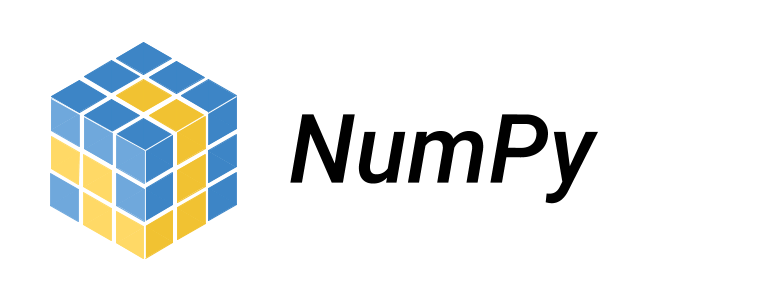
\includegraphics[scale=0.15]{./Imagenes/numpy.png}
\end{figure}
Su característica más potente es que puede trabajar con matrices de $n$ dimensiones. Ofrece funciones básicas de algebra lineal, transformada de Fourier, capacidades avanzadas con números aleatorios, y herramientas de integración con otros lenguajes de bajo nivel como Fortran, C y C++.
\end{frame}
\begin{frame}
\frametitle{Paquete \texttt{scipy}}
\begin{figure}
    
\includegraphics[scale=0.15]{./Imagenes/scipy.png}
\end{figure}
\funcionazul{scipy} está construida sobre la librería \funcionazul{numpy}. Es una de las más útiles por la gran variedad que tiene de módulos de alto nivel sobre ciencia e ingeniería, como transformada discreta de Fourier, álgebra lineal, funciones especiales y matrices de optimización.
\end{frame}
\begin{frame}
\frametitle{Paquete \texttt{matplotlib}}
\frametitle{Paquete \texttt{numpy}}
\begin{figure}
    
\includegraphics[scale=0.15]{./Imagenes/matplotlib.png}
\end{figure}
Es una librería de gráficos, desde histogramas, hasta gráficos de líneas o mapas de color. También se pueden usar comandos de \LaTeX para agregar expresiones matemáticas a la gráfica.
\end{frame}
\begin{frame}
\frametitle{Paquete \texttt{pandas}}
\begin{figure}
    
\includegraphics[scale=0.15]{./Imagenes/pandas.png}
\end{figure}
Se utiliza para operaciones y manipulaciones de datos estructurados. Es muy habitual usarlo en la fase de depuración y preparación de los datos. 
\end{frame}
\begin{frame}
\frametitle{Paquete \texttt{seaborn}}
\begin{figure}
    
\includegraphics[scale=0.25]{./Imagenes/seaborn.png}
\end{figure}
Está basada en \funcionazul{matplotlib}, se usa para hacer más atractivos los gráficos e información estadística en \python.
\\
\bigskip
Su objetivo es darle una mayor relevancia a las visualizaciones, dentro  de las tareas de exploración e interpretación de los datos.
\end{frame}
\section{Graficación con \python}
\frame{\tableofcontents[currentsection, hideothersubsections]}
\subsection{Librería para graficación}
\begin{frame}
\frametitle{Graficación con \python}
Una buena parte del trabajo que tendremos que hacer como físicos es utilizar un conjunto de datos que por si solos, no van a darnos información sobre un modelo o un fenómeno, por ello, será necesario usar gráficas.
\\
\bigskip
De tal manera que contemos con elementos para dar una interpretación de los resultados obtenidos con un código.
\end{frame}
\begin{frame}
\frametitle{Módulo de graficación}
\python\ incluye un módulo de graficación bastante versátil para generar gráficas y exportarlas a diferentes tipos de archivos.
\\
\medskip
La librería se llama \funcionazul{matplotlib} que contiene un conjunto de funciones propias para crear gráficas. Haremos algunos ejercicios sencillos para demostrar su potencia.
\end{frame}
\begin{frame}
\frametitle{El módulo \texttt{pyplot}}
Consideremos que \funcionazul{matplotlib} es un paquete entero, y \funcionazul{matplotlib.pyplot} es una colección de funciones de estilo.
\\
\bigskip
\pause
Cada instrucción \funcionazul{pyplot} aplica un cambio a una figura: por ejemplo, crear una figura, crear un área de trazado en una figura, trazar algunas líneas en un área de trazado, decorar con etiquetas, etc.
\end{frame}
\subsection{Gráficas básicas}
\begin{frame}[fragile]
\frametitle{Código para el Ejercicio 1}
\begin{lstlisting}[style=codigopython, caption=Gráfica básica]
import matplotlib.pyplot as plt

plt.plot([1, 2, 3, 4])
plt.ylabel('algunos numeros')
plt.show()
\end{lstlisting}
\end{frame}
\begin{frame}[fragile]
\frametitle{Gráfica que se obtiene en el Ejercicio 1}
\begin{figure}
	\centering
	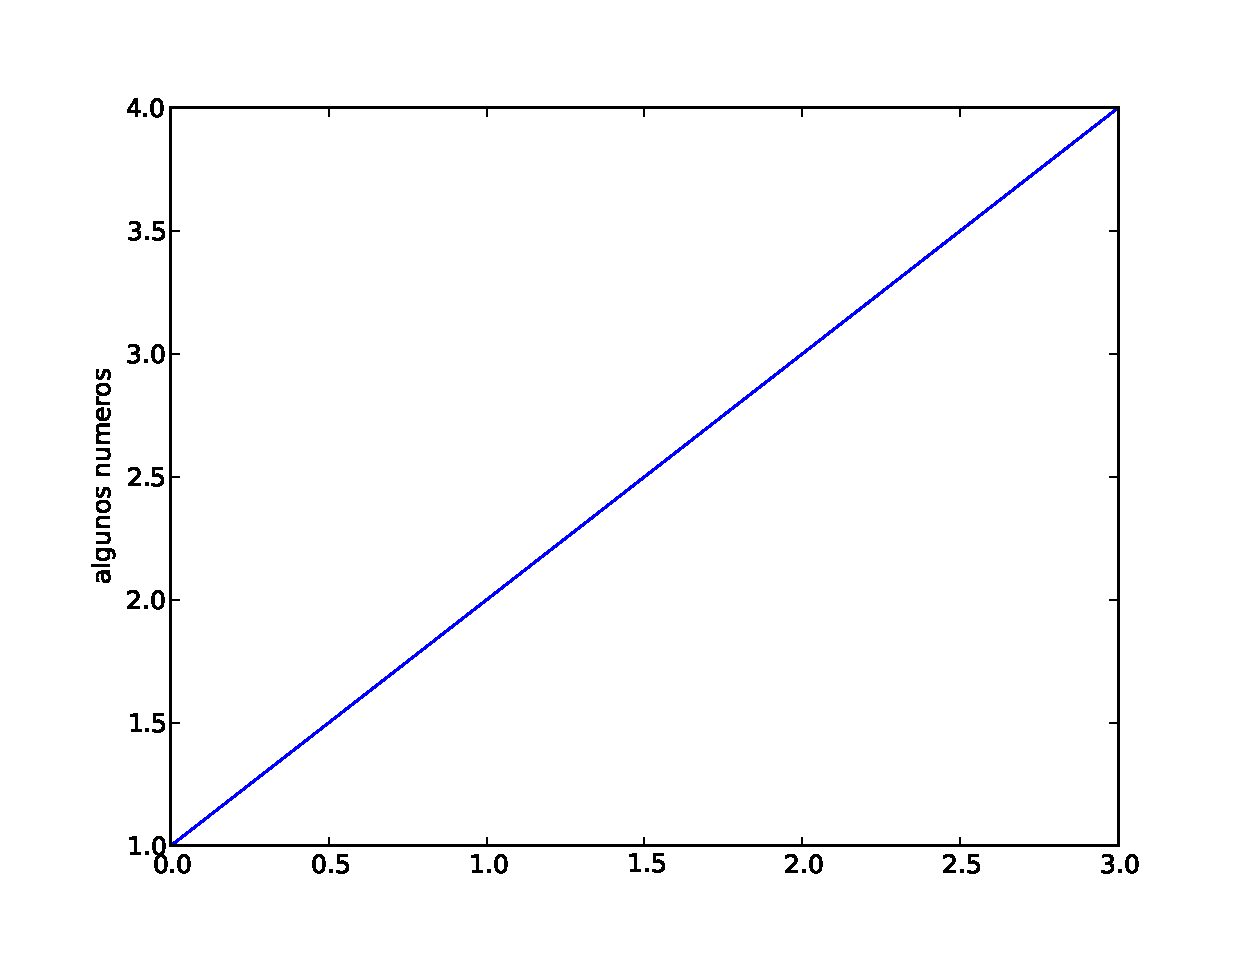
\includegraphics[scale=0.35]{Imagenes/plotEjercicio1.eps}
	\caption{Gráfica obtenida por el primer código.}
\end{figure}
\end{frame}
\begin{frame}[fragile]
\frametitle{Sobre la gráfica obtenida}
Viendo la gráfica anterior que obtuvimos con \funcionazul{matplotlib}, te estarás preguntando: \textcolor{red}{ ¿por qué tenemos en el eje $x$ el rango $0-3$, mientras que en el eje $y$ el rango va de  $1-4$?}
\end{frame}
\begin{frame}
\frametitle{Respuesta}
Cuando proporcionamos una única lista o matriz en el comando \funcionazul{plot(\ )}, entonces \funcionazul{matplotlib} asume que es una secuencia de valores para la variable $y$, por lo que genera automáticamente los valores para la variable $x$ para nosotros, graficando entonces dos variables $(x, y)$. 
\end{frame}
\begin{frame}
\frametitle{Respuesta}	
Como los índices en \python\ comienzan en $0$, el conjunto de datos \emph{(vector)} para la variable $x$ por defecto tiene la misma longitud que la variable $y$, pero inicia en $0$. 
\\
\bigskip
De ahí que el conjunto de datos para la variable $x$ son $[0, 1, 2, 3]$.
\end{frame}
\begin{frame}[fragile]
\frametitle{Código para el Ejercicio 2}
\begin{lstlisting}[style=codigopython]
import matplotlib.pyplot as plt

plt.plot([1,2,3,4], [1,4,9,16], 'ro')
plt.axis([0,6,0,20])
plt.show()
\end{lstlisting}
\end{frame}
\begin{frame}[fragile]
\frametitle{Gráfica que se obtiene en el Ejercicio 2}
\begin{figure}
    \centering
	\includegraphics[scale=0.35]{Imagenes/plotEjercicio2.eps}
 	\caption{Gráfica obtenida con el segundo código.}
\end{figure}
\end{frame}
\begin{frame}[fragile]
\frametitle{Sobre la segunda gráfica}
Se han introducido dos listas en el argumento de \funcionazul{plot (\ )}, que corresponden a los valores para los pares $(x, y)$.
\\
\bigskip
Es importante señalar que para generar una gráfica, tanto la variable $x$ como la variable $y$, \emph{deben de contar con el mismo número de puntos.}
\end{frame}
% \begin{frame}[fragile]
% \frametitle{Sobre la segunda gráfica}
% También se agregó una cadena \funcionazul{'ro'}, que modifica la gráfica: no tenemos una línea continua, se muestran sólo los puntos, éstos son de color rojo, entonces, esta modificación se obtuvo de \textcolor{red}{'r'} = red (rojo), mientras que \textcolor{blue}{'o'} = círculo con color de relleno.
% \end{frame}
% \begin{frame}[fragile]
% \frametitle{Elementos incorporados}
% \texttt{
% plt.plot(\tikzmark{a1}[1,2,3,4],\tikzmark{a2}[1,4,9,16],\tikzmark{a3}'ro')
% \\
% \bigskip
% \vspace{1.5cm}
% plt.plot(\tikzmark{b1}x,\tikzmark{b2}y, \tikzmark{b3}'tipolinea-marca')
% }
% \begin{tikzpicture}[remember picture,overlay]
%     \path[draw=blue,thick,->] ([xshift=2mm, yshift=3mm]b1) -- ([xshift=1cm, yshift=-2mm]a1);
%     \path[draw=blue,thick,->] ([xshift=2mm, yshift=3mm]b2) -- ([xshift=1cm, yshift=-2mm]a2);
%     \path[draw=blue,thick,->] ([xshift=2cm, yshift=3mm]b3) -- ([xshift=3mm, yshift=-2mm]a3);

% \end{tikzpicture}
% \end{frame}
% % \begin{frame}[fragile]
% % \frametitle{Elementos incorporados}
% % \texttt{
% % plt.axis(\tikzmark{a1}[0, 6, \tikzmark{a2}0, 20])
% % \\
% % \bigskip
% % \vspace{1.5cm}
% % plt.axis(\tikzmark{b1}x1, x2, \tikzmark{b2}y1, y2)
% % }
% % \begin{tikzpicture}[remember picture,overlay]
% %     \path[draw=blue,thick,->] ([xshift=2mm, yshift=3mm]b1) -- ([xshift=5mm, yshift=-2mm]a1);
% %     \path[draw=blue,thick,->] ([xshift=2mm, yshift=3mm]b2) -- ([xshift=2mm, yshift=-2mm]a2);
% % \end{tikzpicture}
% % \end{frame}
% % \begin{frame}
% % \frametitle{Ejercicio 2}
% % \begin{figure}
% % 	\centering
% % 	\includegraphics[scale=0.35]{Imagenes/plotEjercicio2.eps}
% % 	\caption{Gráfica obtenida con dos listas de números. Nótese que los puntos no están unidos entre sí.}
% % \end{figure}
% % \end{frame}
% \begin{frame}[fragile]
% \frametitle{Sobre la segunda gráfica: cadena de formato}
% Por cada par de argumentos $(x, y )$, existe un tercer argumento opcional, que es la cadena de formato que indica el color y tipo de línea.
% \\
% \bigskip
% Las letras y los símbolos de la cadena de formato concatenan una cadena de color con una cadena que define el estilo de línea.

% \end{frame}
\begin{frame}[fragile]
\frametitle{Sobre la segunda gráfica: cadena de formato}
La cadena de formato por defecto es \verb|'b-'|, que corresponde al color azul (\verb|b = blue|). Es por ello que en la gráfica 1, los puntos quedaron unidos con la línea azul.
\\
\bigskip
En la gráfica 2, usamos la cadena \verb|'ro'|, que nos generó los círculos de color rojo (\verb|r = red|).
\end{frame}
\begin{frame}[fragile]
\frametitle{Cadena de formato para el color}
\begin{minipage}{0.4\linewidth}
\fontsize{12}{10}\selectfont
\begin{tabular}{l | l}
caracter & color \\ \hline
\verb|'b'| & azul \\ \hline
\verb|'g'| & verde \\ \hline
\verb|'r'| & rojo \\ \hline
\verb|'c'| & cyan \\ \hline
\verb|'m'| & magenta \\ \hline
\verb|'y'| & amarillo \\ \hline
\verb|'k'| & negro \\ \hline
\verb|'w'| & blanco
\end{tabular}
\end{minipage}
\hspace{0.3cm}
\begin{minipage}{0.5\linewidth}
\fontsize{13}{12}\selectfont
Esta lista presenta la correspondiente letra para incluir en la cadena de formato de color en la función \funcionazul{plot(\ )}, es posible personalizar el color a mostrar: consultando la documentación de \funcionazul{matplotlib}.
\end{minipage}
\end{frame}
\begin{frame}[fragile]
\frametitle{Cadena de formato para el tipos de línea}
\begin{minipage}{0.4\linewidth}
\fontsize{10}{10}\selectfont
\begin{tabular}{l | l}
carácter & descripción \\ \hline
\verb|'-'|	& línea sólida \\ \hline
\verb|'--'| & línea cortada \\ \hline
\verb|'-.'| & línea-punto \\ \hline
\verb|':'|	& línea de puntos \\ \hline
\verb|'.'|	& marca de punto \\ \hline
\verb|','|	& marca de pixel \\ \hline
\verb|'o'|	& marca de círculo \\ \hline
\verb|'v'|	& marca de triángulo hacia abajo \\ \hline
\verb|'^'|	& marca de triángulo hacia arriba
\end{tabular}
\end{minipage}
\hspace{0.7cm}
\begin{minipage}{0.5\linewidth}
\fontsize{13}{12}\selectfont
Esta lista muestra el caracter para definir el tipo de línea en el argumento de la función la función \funcionazul{plot(\ )}.
\end{minipage}
\end{frame}
\begin{frame}
\frametitle{Alcance de \texttt{matplotlib}}
El paquete \funcionazul{matplotlib} se limita a trabajar con listas, por lo que su uso sería bastante acotado para el procesamiento y análisis numérico.
\\
\medskip
Por lo general, se utilizan los arreglos del paquete \funcionazul{numpy}.
\end{frame}
\begin{frame}
\frametitle{Extendiendo \texttt{matplotlib}}
De hecho, todas las secuencias se convierten en arreglos de \funcionazul{numpy} internamente.
\\
\medskip
El siguiente ejemplo ilustra un trazado de líneas con varios estilos diferentes en una sola instucción utilizando arreglos.
\end{frame}
\begin{frame}[fragile]
\frametitle{Código para el Ejercicio 3}
\begin{lstlisting}[style=codigopython]
import numpy as np
import matplotlib.pyplot as plt

t = np.arange(0., 5., 0.2)
plt.plot(t, t, 'r--', t, t**2, 'bs', t, t**3, 'g^')
plt.show()
\end{lstlisting}
\end{frame}
% \begin{frame}[fragile]
% \frametitle{Elementos en el código}
% \texttt{
% t = np.arange\tikzmark{a1}(0., \tikzmark{b1}5., \tikzmark{c1}0.2)
% \\
% \bigskip
% \vspace{1.5cm}
% t = np.arange(\tikzmark{a2}inicio, \tikzmark{b2}fin, \tikzmark{c2}paso)
% }
% \begin{tikzpicture}[remember picture,overlay]
%     \path[draw=magenta,thick,->] ([xshift=2mm, yshift=3mm]a2) -- ([xshift=5mm, yshift=-2mm]a1);
%     \path[draw=magenta,thick,->] ([xshift=2mm, yshift=3mm]b2) -- ([xshift=2mm, yshift=-2mm]b1);
%     \path[draw=magenta,thick,->] ([xshift=2mm, yshift=3mm]c2) -- ([xshift=5mm, yshift=-2mm]c1);
% \end{tikzpicture}
% \end{frame}
\begin{frame}[fragile]
\begin{figure}
	\centering
  	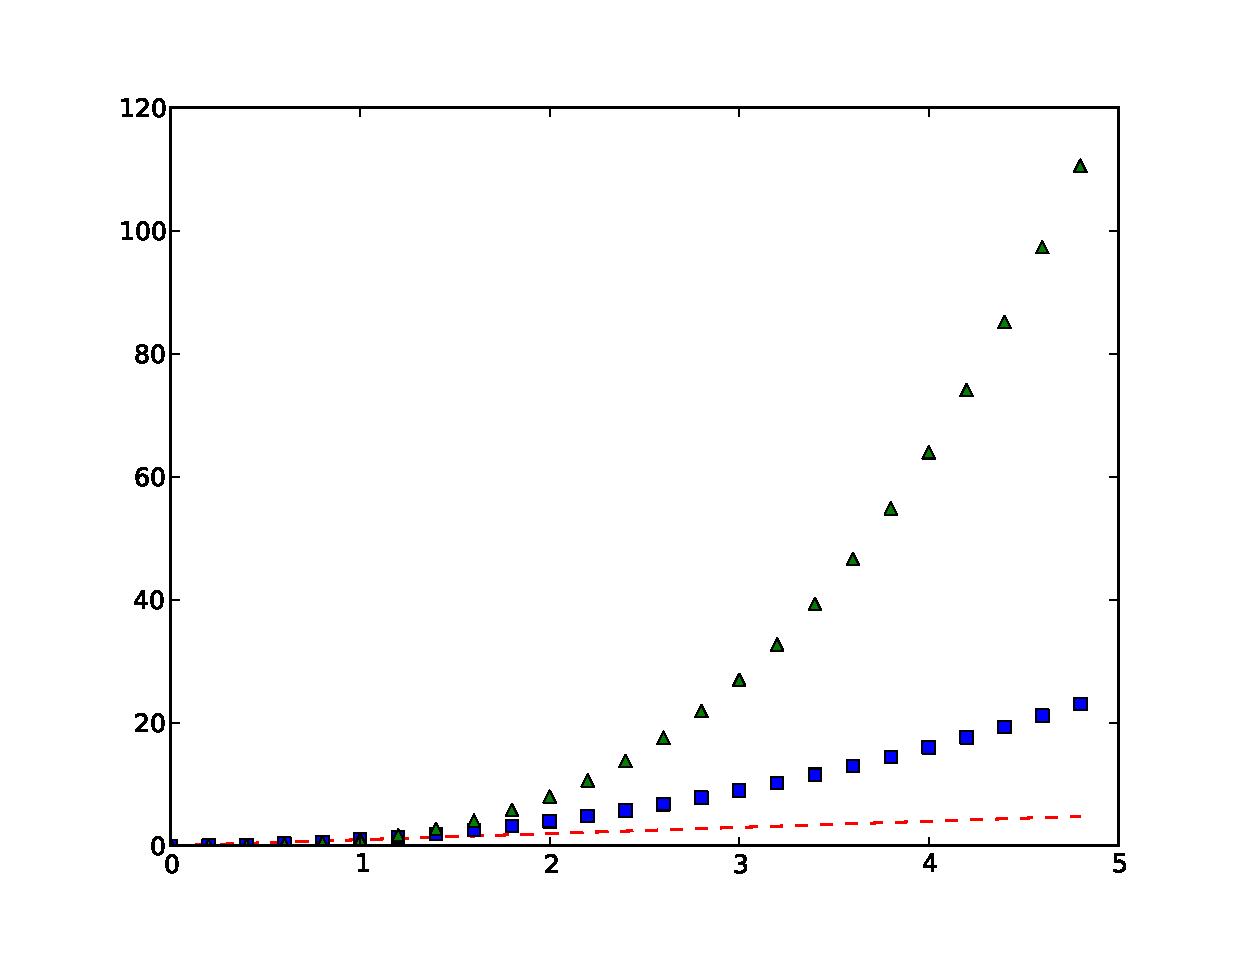
\includegraphics[scale=0.5]{Imagenes/plotEjercicio3.eps}
  	\caption{Gráfica con tres curvas.}
\end{figure}
\end{frame}
\subsection{Trabajando con subplots}
\begin{frame}
\frametitle{Los subplots en \python}
Ya hemos generado una gráfica que contenga un trazo para una función en particular.
\\
\bigskip
Pero hay que considerar que a veces necesitaremos mostrar dos (o más) gráficas dentro de la misma ventana), en éste caso usaremos los \emph{subplots}.
\end{frame}
\begin{frame}[allowframebreaks, fragile]
\frametitle{Código para el Ejercicio 4}
\begin{lstlisting}[style=codigopython]
import numpy as np
import matplotlib.pyplot as plt

def f(t):
    return np.exp(-t) * np.cos(2*np.pi*t)

tA_1_B = np.arange(0.0, 5.0, 0.1)
tA_2_B = np.arange(0.0, 5.0, 0.02)

plt.figure(1)
plt.subplot(211)
plt.plot(tA_1_B, f(tA_1_B), 'bo', tA_2_B, f(tA_2_B), 'k')

plt.subplot(212)
plt.plot(tA_2_B, np.cos(2*np.pi*tA_2_B), 'r--')

plt.show()
\end{lstlisting}
\end{frame}
\begin{frame}[fragile]
\begin{figure}
	\centering
	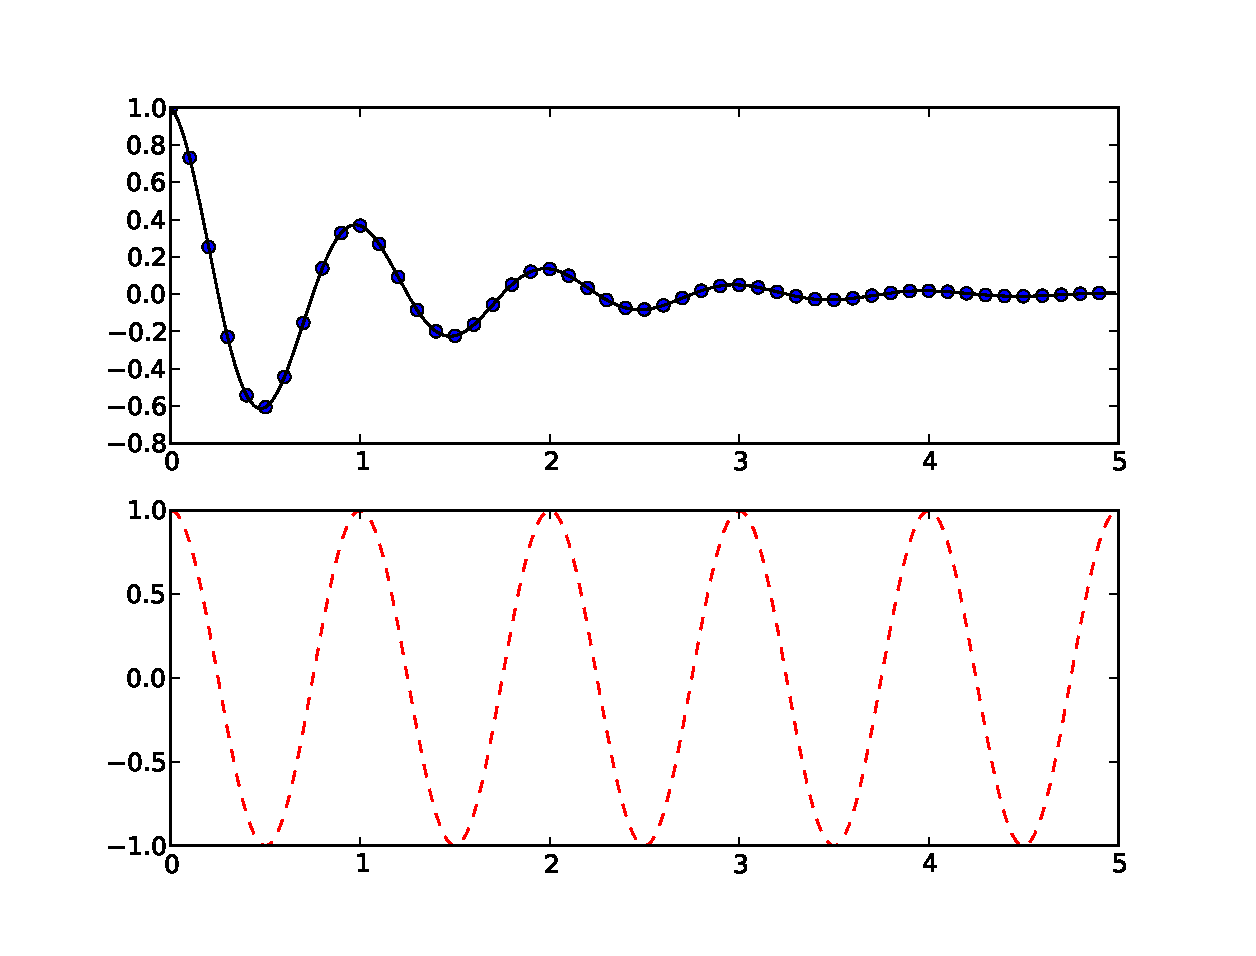
\includegraphics[scale=0.5]{Imagenes/plotEjercicio4.eps}
\end{figure}
\end{frame}
\begin{frame}
\frametitle{Especificar los \texttt{subplots}}
El comando \funcionazul{figure(\ )} aquí es opcional, ya \funcionazul{figure(1)} se crea de forma predeterminada, así mismo \funcionazul{subplot(111)} se crea de forma predeterminada si no se especifica manualmente un eje.
\end{frame}
\begin{frame}
\frametitle{Especificar los \texttt{subplots}}
La función \funcionazul{figure1()} está avisando el uso de una ventana para mostrar la gráfica.
\\
\bigskip
La función \funcionazul{subplot()} requiere que se señale como parámetros: \texttt{(numrows, numcols, fignum)} donde \texttt{fignum} varía en rango de $1$ a \texttt{numrows * numcols}.
\end{frame}
\begin{frame}
\frametitle{Especificar los \texttt{subplots}}
Las comas en la función \funcionazul{subplot()} son opcionales si \texttt{numrows * numcols} $<10$. 
\\
\bigskip
Por tanto \funcionazul{subplot(211)} es idéntica a la \funcionazul{subplot(2,1,1)}.
\end{frame}
\begin{frame}[allowframebreaks, fragile]
\frametitle{Código para el Ejercicio 5}
\begin{lstlisting}[style=codigopython]
import matplotlib.pyplot as plt
import numpy as np

xA_1_B = np.linspace(0, 18, 200)
xA_2_B = np.linspace(0, 5, 100)

plt.figure(1)                
plt.subplots_adjust(hspace=0.5)

plt.subplot(211)        
plt.plot([1, 2, 3])
plt.title('Ventana A_1_B - Subplot A_1_B')

plt.subplot(212)         
plt.plot(xA_1_B, np.cos(xA_1_B))
plt.title('Ventana A_1_B - Subplot A_2_B')

plt.figure(2)                
plt.plot(xA_2_B, np.exp(xA_2_B))           
plt.title('Ventana A_2_B')

plt.show()
\end{lstlisting}
\end{frame}
\begin{frame}[fragile]
\frametitle{Primera ventana con dos subplots}
\begin{figure}
	\centering
    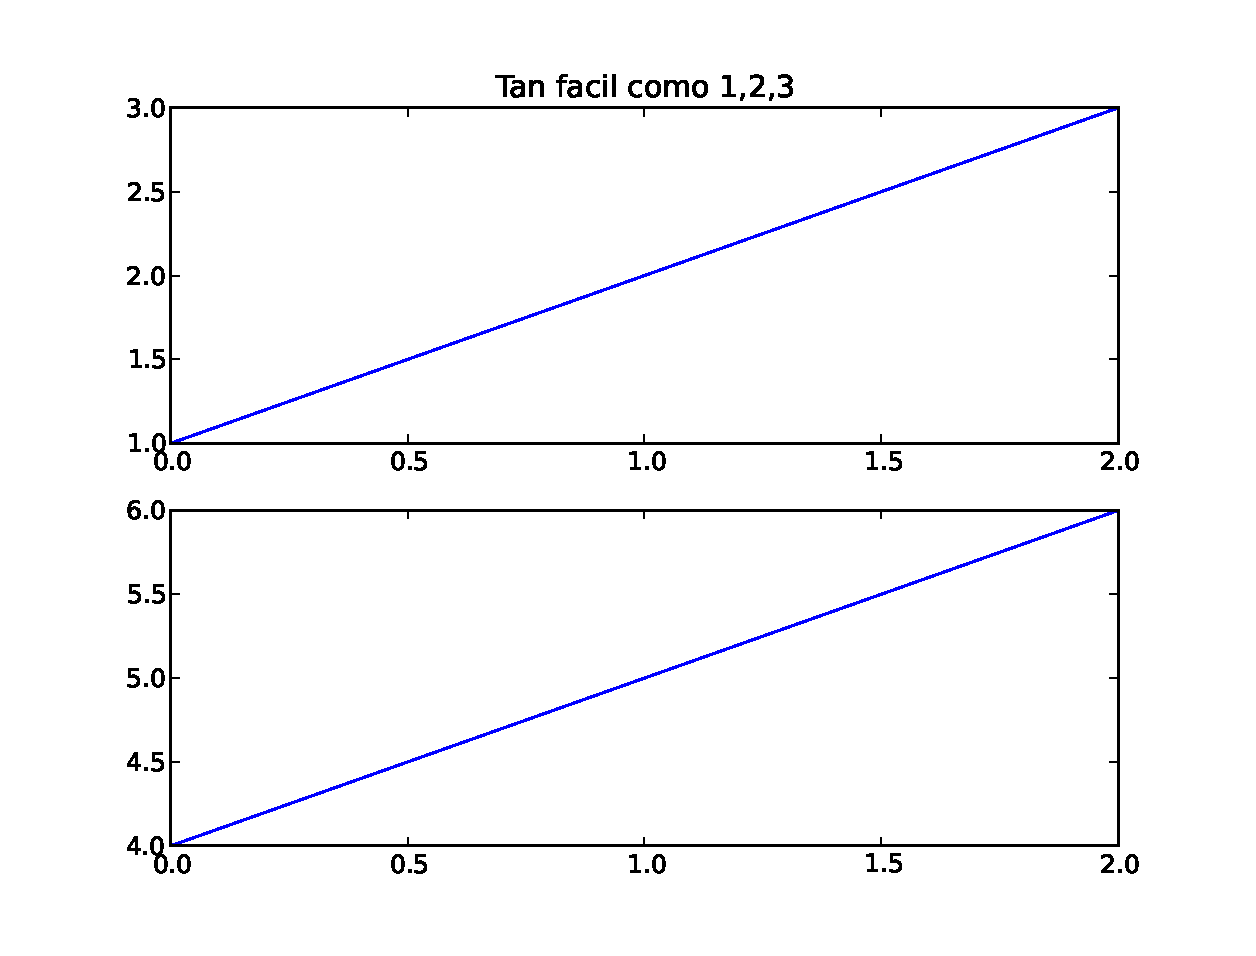
\includegraphics[scale=0.6]{Imagenes/plotEjercicio5_1.eps}
\end{figure}
\end{frame}
\begin{frame}[fragile]
\frametitle{Segunda ventana con una gráfica}
\begin{figure}
    \centering
    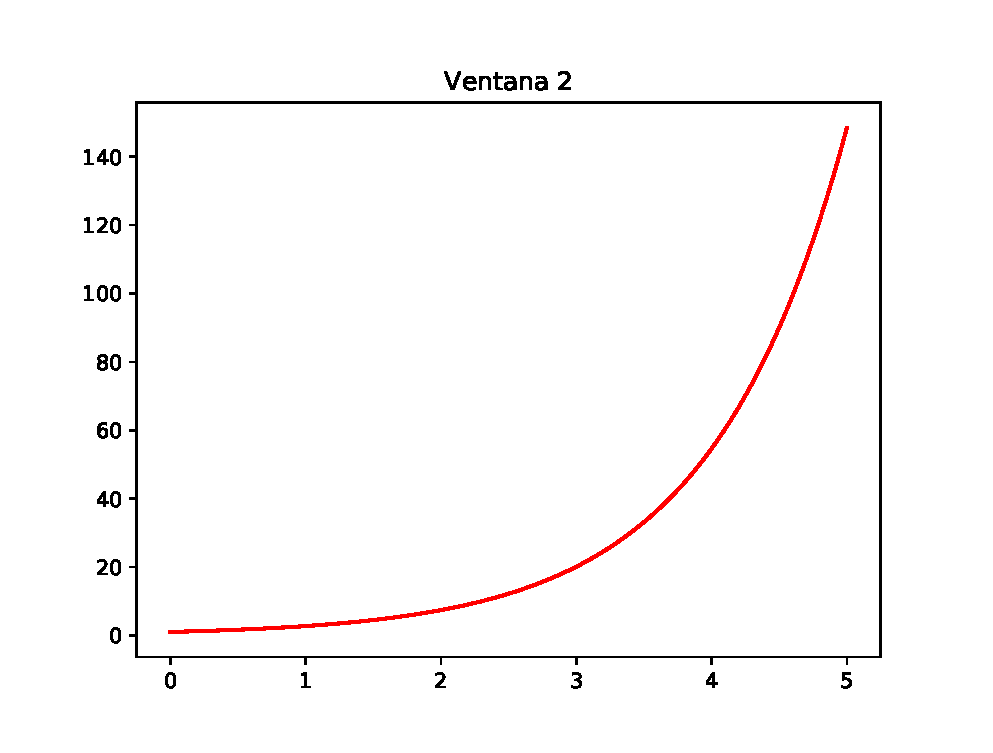
\includegraphics[scale=0.6]{Imagenes/plotEjercicio5_2.eps}
\end{figure}
\end{frame}
\subsection{Recursos para \texttt{matplotlib}}
\begin{frame}
\frametitle{Más recursos para graficar con \python}
Lo que hemos visto es una revisión muy básica y general de cómo generar una gráfica con \python.
\end{frame}
\begin{frame}
\frametitle{Más recursos para graficar con \python}
Hay una enorme cantidad de información sobre \funcionazul{matplotlib}, que encontrarás en la página oficial de la librería, así como bastante documentación, ejemplos y elementos para extender completamente esta herramienta.
\end{frame}
\begin{frame}
Se les proporcionará una guía breve de graficación, con la intención de que revisen casos prácticos aplicados a la física.
\\
\bigskip
Para cada gráfica que usemos más adelante en el curso, tendrán oportunidad de agregar más elementos que ustedes consideren.
\end{frame}
\begin{frame}
\frametitle{Ejemplos de tipos de gráficas}
\begin{figure}
	\centering
	\only<1>{
	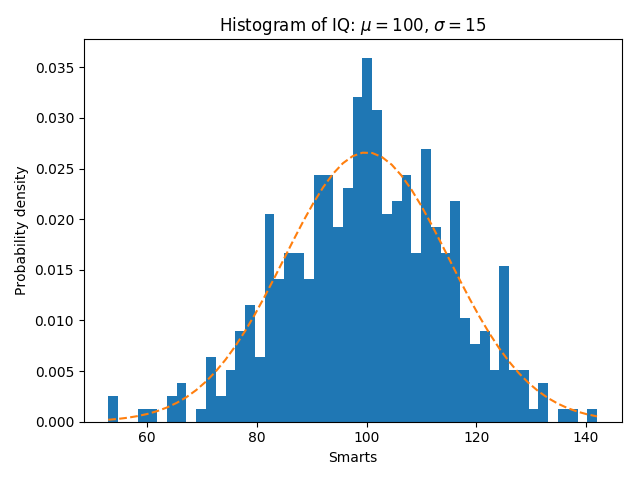
\includegraphics[scale=0.5]{Imagenes/sphx_glr_histogram_features_001.png}
	\caption{Histograma}
	}
	\only<2>{
	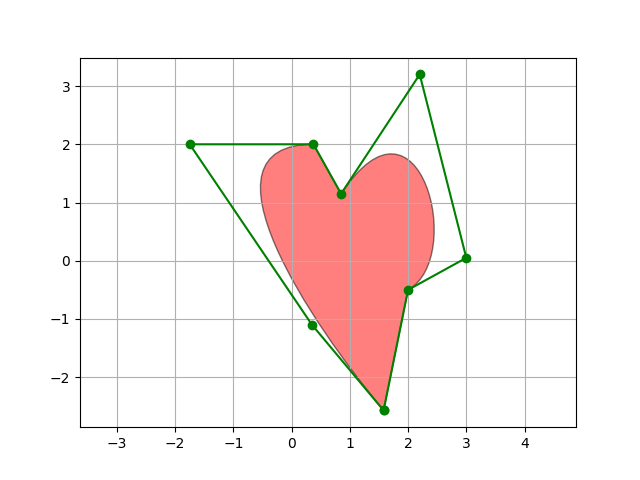
\includegraphics[scale=0.5]{Imagenes/sphx_glr_path_patch_001.png}
	\caption{Contorno}
	}
	\only<3>{
	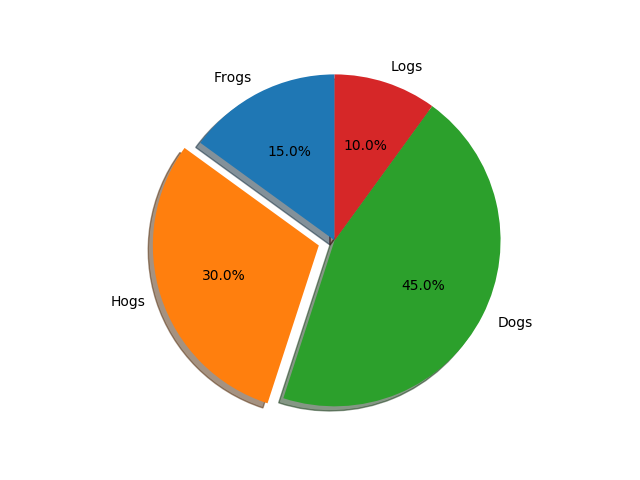
\includegraphics[scale=0.5]{Imagenes/sphx_glr_pie_features_001.png}
	\caption{Pastel}
	}
	\only<4>{
	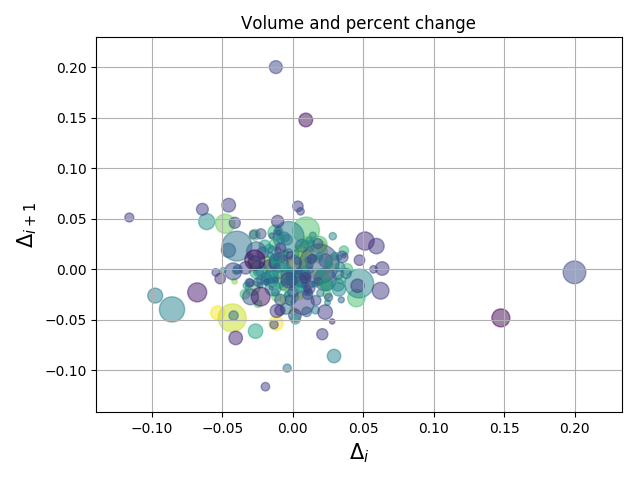
\includegraphics[scale=0.5]{Imagenes/sphx_glr_scatter_demo2_001.png}
	\caption{Dispersión}
	}
	\only<5>{
	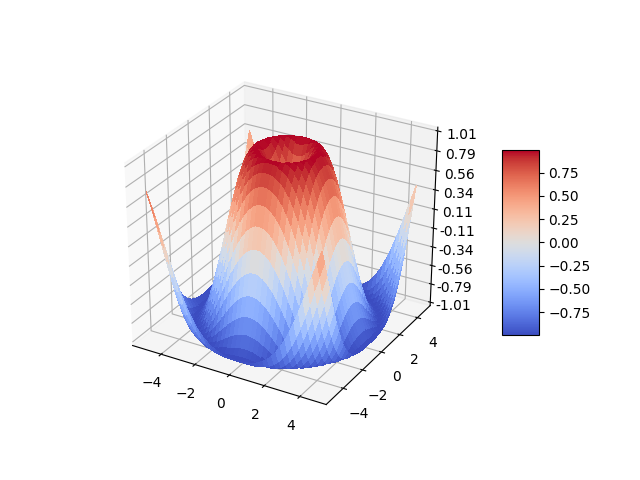
\includegraphics[scale=0.5]{Imagenes/sphx_glr_surface3d_001.png}
	\caption{Superficie 3D}
	}
	\only<6>{
	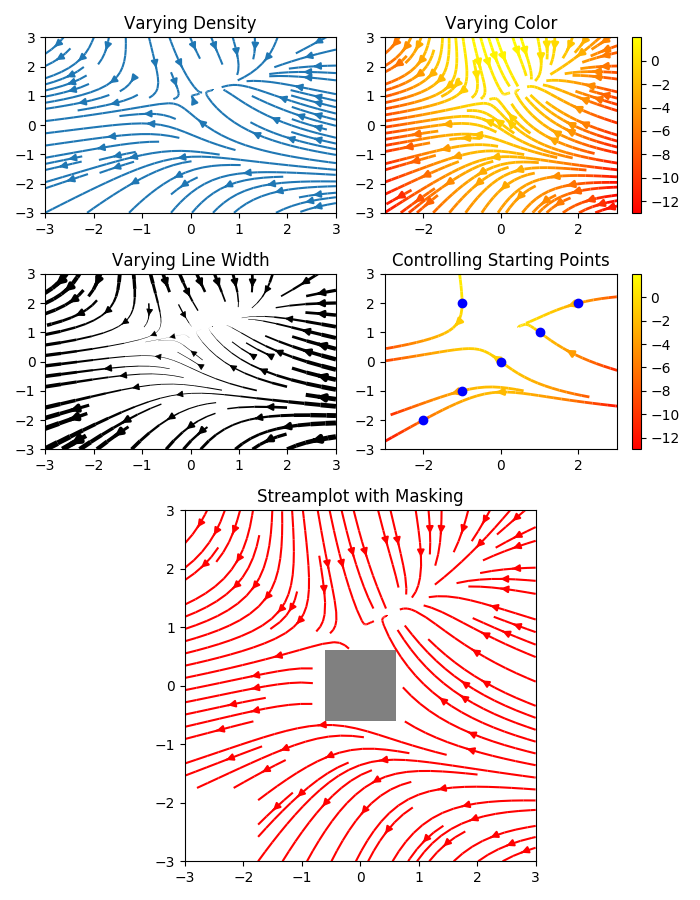
\includegraphics[scale=0.25]{Imagenes/sphx_glr_plot_streamplot_001.png}
	\caption{Campos vectoriales}
	}
\end{figure}
\end{frame}
\section{Ejercicio de Mecánica}
% \frame{\tableofcontents[currentsection, hideothersubsections]}
% \subsection{El oscilador armónico}
% \begin{frame}
% \frametitle{Un primer problema de Mecánica}
% Supongamos que tenemos una partícula de masa $m$ que está confinada a moverse a lo largo del eje $x$, bajo una fuerza $f(x)$. Sabemos de la ley de Newton que
% \begin{equation}\label{Eqfuerza}
% f = ma = m \dfrac{dv}{dt}
% \end{equation}
% donde $a$ es la aceleración y $v$ la velocidad de la partícula respectivamente, $t$ es el tiempo.
% \end{frame}
% \begin{frame}
% \frametitle{Un primer problema de Mecánica}
% Si dividimos el tiempo en pequeños intervalos iguales $\tau = t_{i + 1} - t_{i}$, sabemos que la velocidad en el tiempo $t_{i}$, está dada de manera aproximada por el promedio de la velocidad en el intervalo de tiempo $[t_{i}, t_{i + 1}]$
% \end{frame}
% \begin{frame}
% \frametitle{Un primer problema de Mecánica}
% Por lo que
% \begin{equation}\label{Eqvelocidad}
% v_{i} \simeq \dfrac{x_{i+1}-x_{i}}{t_{i+1}-t_{i}} = \dfrac{x_{i+1}-x_{i}}{\tau}
% \end{equation}
% \end{frame}
% \begin{frame}
% \frametitle{Un primer problema de Mecánica}
% La aceleración de la partícula es aproximadamente el promedio de la aceleración en el mismo intervalo
% \begin{equation}\label{Eqaceleracion}
% a_{i} \simeq \dfrac{v_{i+1}-v_{i}}{t_{i+1}-t_{i}} = \dfrac{v_{i+1}-v_{i}}{\tau}
% \end{equation}
% donde $\tau$ es muy pequeño.
% \end{frame}
% \begin{frame}
% \frametitle{Hallar la posición y velocidad}
% El algoritmo más sencillo para determinar la posición y velocidad de la partícula en el tiempo $t_{1i+1}$, a partir de las cantidades correspondientes al tiempo $t_{i}$, se obtiene luego de combinar las ecuaciones (\ref{Eqfuerza}), (\ref{Eqvelocidad}) y (\ref{Eqaceleracion}), por lo que
% \begin{eqnarray}
% x_{i+1} &=& x_{i} + \tau v_{i} \label{Eqposicion} \\
% v_{i+1} &=& v_{i} + \dfrac{\tau}{m} f_{i} \label{Eqvelocidadr}
% \end{eqnarray}
% donde $f_{i} = f(x_{i})$
% \end{frame}
% \begin{frame}
% \frametitle{Hallar la posición y velocidad}
% Si se proporcionan la posición inicial y la velocidad inicial de la partícula, para luego calcular las cantidades correspondientes en algún momento posterior (problema de valor inicial), podemos obtenerlas de forma recursiva a partir del algoritmo dado en las ecuaciones (\ref{Eqposicion}) y (\ref{Eqvelocidadr}).
% \end{frame}
% \begin{frame}
% \frametitle{Ejercicio 1: Oscilador mecánico}
% Por simplicidad, consideremos que la fuerza es $f(x) = -kx$, donde $k$ es la constante del resorte. Usemos $m=k=1$.
% \\
% \bigskip
% \pause
% Queremos describir la posición y velocidad de la partícula en un intervalo de tiempo de 100 segundos.
% \\
% \bigskip
% \pause
% Las condiciones iniciales son las siguientes: $x(t=0) = 0$ y $v(t=0) = 1$.
% \end{frame}
% \begin{frame}[<+->]
% \frametitle{Resolviendo el problema con Python}
% ¿Qué es lo que tenemos?
% \begin{itemize}
% \item El intervalo de tiempo de $[0,100]$ segundos.
% \item La posición inicial y velocidad inicial.
% \item Las expresiones para calcular los $x_{i+1}$ y $v_{i+1}$
% \end{itemize}
% \visible<4->{¿Qué nos falta?}
% \end{frame}
% \begin{frame}[fragile]
% \frametitle{Lo que nos falta}
% \begin{itemize}[<+->]
% \item Calcular la posición y velocidad para cada segundo en el intervalo $[0,100]$.
% \item Guardar esos valores en un algún lado.
% \item Graficar los resultados.
% \end{itemize}
% \end{frame}
% \begin{frame}[fragile]
% \frametitle{Uso de los módulos para nuestro programa}
% Para graficar con el módulo \funcionazul{matplotlib} incluido en \python, necesitamos llamar a la librería \funcionazul{pyplot}, para acortar la escritura, usamos un \emph{alias}, en este caso \texttt{plt}.
% \begin{lstlisting}
% import matplotlib.pyplot as plt
% from math import pi
% \end{lstlisting}
% \end{frame}
% \begin{frame}[fragile]
% \frametitle{Usando lo que conocemos}
% \begin{lstlisting}
% n = 100

% x = []
% v = []

% dt = 2* pi/n

% x.append(0)
% v.append(1)
% \end{lstlisting}
% \end{frame}
% \begin{frame}[fragile]
% \frametitle{Ciclo de iteración para los nuevos valores}
% Como la fuerza en este caso es del tipo $f(x) = -k \; x$, tenemos un cambio de signo en el segundo sumando de $vi$.
% \pause
% \begin{lstlisting}
% for i in range(n-1):
%     xi = x[i] + v[i]*dt
%     vi = v[i] - x[i]*dt
    
%     x.append(xi)
%     v.append(vi)
% \end{lstlisting}
% \end{frame}
% \begin{frame}
% \frametitle{Almacenando los valores nuevos}
% Conforme se itera en el ciclo \funcionazul{for ... in}, se obtienen nuevos valores tanto de la posición como de la velocidad, y se almacenan en las respectivas listas.
% \\
% \bigskip
% Desplegar el contenido de las dos columnas en la termina, no nos brinda una forma de apreciar el resultado, entonces lo que haremos, es graficar esos datos.
% \end{frame}
% \begin{frame}[fragile]
% \frametitle{Crear la gráfica}
% \begin{lstlisting}
% plt.plot(x, "ro-", label="Posicion")
% plt.plot(v, "b+-", label="Velocidad")
% plt.legend(loc="upper right")
% plt.xlabel("tiempo")
% plt.show()
% \end{lstlisting}
% \end{frame}
% \begin{frame}
% \frametitle{Resultado del problema}
% \begin{figure}
% 	\centering
% 	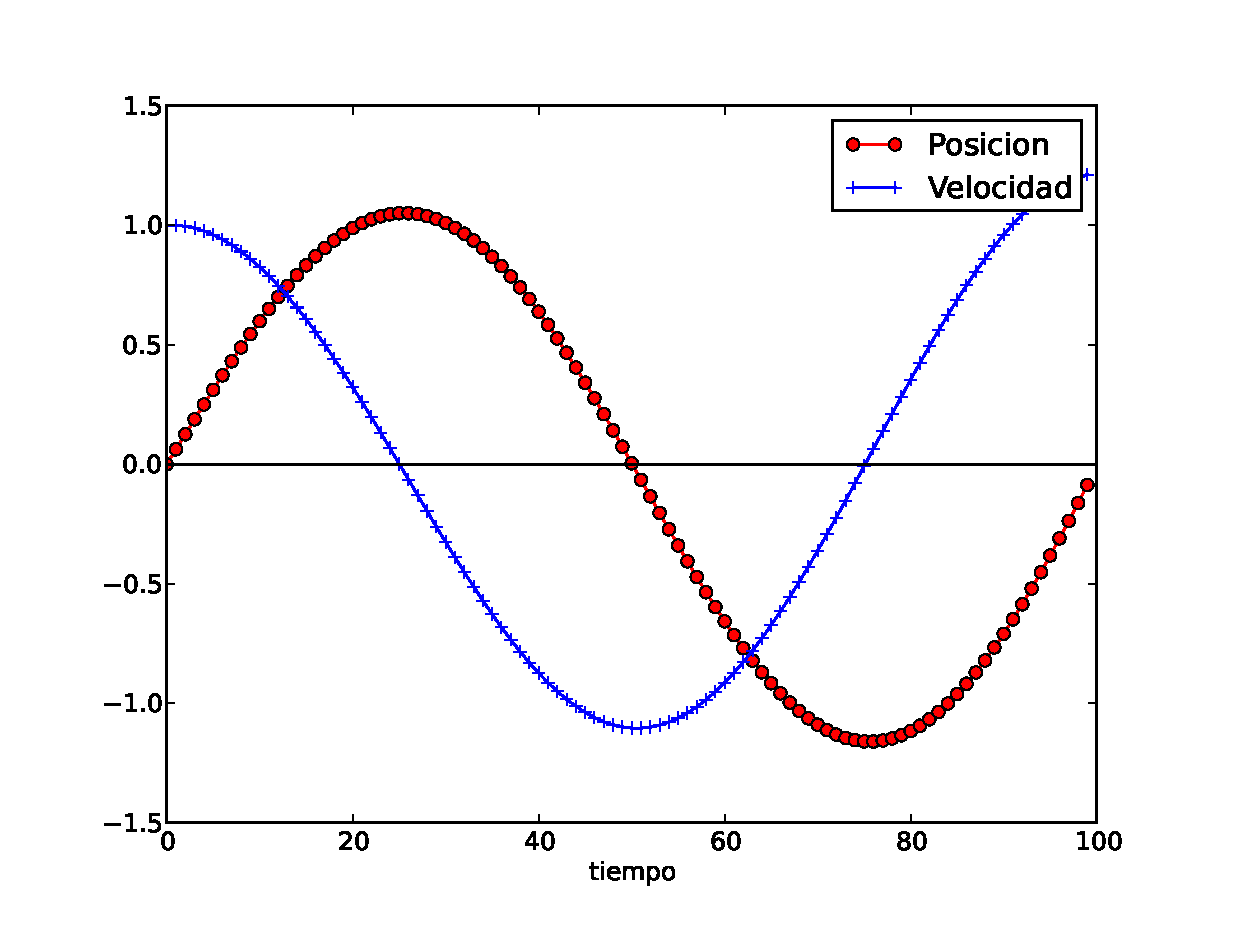
\includegraphics[scale=0.5]{Imagenes/EjerMecanica01.eps} 
% \end{figure}
% \end{frame}
\subsection{Un problema de mecánica}
\begin{frame}
\frametitle{Ejercicio: movimiento en bicicleta}
La bicicleta es un medio muy eficiente de transporte, este es un hecho bien conocido por cualquier persona que monta una. 
\\
\bigskip
Nuestro objetivo en este ejercicio es comprender los factores que determinan la velocidad máxima de una bicicleta y estimar la velocidad de un caso real.
\end{frame}
\begin{frame}
\frametitle{Ejercicio: Caso sin fricción}
Comenzaremos haciendo caso omiso de la fricción; tendremos que añadirlo al final, por supuesto, pero debemos primero entender cómo lidiar con el caso más simple y sin fricción.
\end{frame}
\begin{frame}
\frametitle{Ecuación de movimiento}
La ecuación de movimiento corresponde a la segunda ley de Newton, que escribimos de la forma
\begin{align}
\dfrac{dv}{dt} = \dfrac{F}{m}
\label{EqNewton2}
\end{align}
\end{frame}
\begin{frame}
\frametitle{Ecuación de movimiento}
\begin{equation*}
\dv{v}{t} = \dfrac{F}{m}
\end{equation*}
donde
\setbeamercolor{item projected}{bg=green!70!black,fg=white}
\setbeamertemplate{enumerate items}[circle]
\begin{enumerate}[<+->]
\fontsize{13}{13}\selectfont
\item $v$ es la velocidad.
\item $m$ es la masa de la combinación de la bicicleta-conductor.
\item $t$ es el tiempo.
\item $F$ es la fuerza en la bicicleta que viene del esfuerzo del conductor (supondremos que la bicicleta se mueve sobre un terreno plano)
\end{enumerate}
\end{frame}
\begin{frame}
\frametitle{Definiendo la fuerza}
Tratar debidamente a la fuerza $F$, se complica por la mecánica de la bicicleta: ya que la fuerza ejercida por el ciclista se transmite a las ruedas por medio del plato, engranajes, cadena, etc.
\\
\medskip
Esto hace que sea muy difícil derivar una expresión exacta para $F$.
\end{frame}
\begin{frame}
\frametitle{Definición alterna de la fuerza}
Sin embargo, hay otra manera de abordar este problema que evita la necesidad de conocer la fuerza.
\\
\medskip
Este enfoque alternativo implica la formulación del problema en términos de la potencia generada por el ciclista.
\end{frame}
\begin{frame}
\frametitle{Comparando la potencia}
Estudios fisiológicos en ciclistas de carreras han demostrado que éstos atletas son capaces de producir una potencia de salida de aproximadamente $400$ watts durante largos períodos de tiempo ($\sim 1$ h)
\end{frame}
\begin{frame}
\frametitle{Usando la potencia generada}
Usando las ideas de trabajo-energía podemos reescribir (\ref{EqNewton2}) como
\begin{align}
\dv{E}{t} = P
\label{EqPotencia}
\end{align}
donde $E$ es la energía total, $P$ es la potencia de salida del ciclista. 
\end{frame}
\begin{frame}
\frametitle{Expresando la velocidad}
Para un trayecto plano la energía es totalmente cinética, es decir,
\begin{align*}
E = \frac{1}{2} m v^{2}
\end{align*}
y además
\begin{align*}
\dv{E}{t} = mv  \left( \dv{v}{t} \right)
\end{align*}
\pause
usando esto en la ec. (\ref{EqPotencia}), resulta
\begin{align}
\dv{v}{t} = \dfrac{P}{mv}
\label{EqPotenciavel}
\end{align}
\end{frame}
\begin{frame}
\frametitle{Expresando la velocidad}
Si $P$ es una constante, la ecuación (\ref{EqPotenciavel}), se puede resolver de manera analítica, rearreglando términos:
\begin{align}
\int_{v_{0}}^{v} v^{\prime} \dd{v^{\prime}} = \int_{0}^{t} \dfrac{P}{m} \dd{t^{\prime}}
\label{EqIntegral}
\end{align}
donde $v_{0}$ es la velocidad de la bicicleta en $t=0$. 
\end{frame}
\begin{frame}
\frametitle{Obteniendo la velocidad}
Integrando ambos lados de la ecuación (\ref{EqIntegral} y resolviendo para $v$, tenemos que la velocidad del ciclista es:
\begin{align}
v = \sqrt{v_{0}^{2} + 2 \: P \: \dfrac{t}{m}}
\label{Eqvres}
\end{align}
\end{frame}
\begin{frame}
\frametitle{Pasando al código}
Como ya tenemos un conjunto de elementos necesarios para resolver el ejercicio, ahora nos enfocamos a traducir en el lenguaje de \python, lo necesario para la solución.
\\
\bigskip
Recuerda que debemos de almacenar los valores nuevos de velocidad, como se calcula un valor nuevo por cada unidad de tiempo, entonces ya tenemos un par de variables para graficar.
\end{frame}
\begin{frame}[allowframebreaks, fragile]
\frametitle{El caso sin fricción}
\begin{lstlisting}[style=codigopython]
import matplotlib.pyplot as plt
from math import sqrt

t = []
v = []
dt, potencia, masa, tmax = 1, 400, 70, 400
nmax = tmax/dt

t.append(0)
v.append(4)

#calculando nuevos valores
for i in range(int(nmax)):
    ti = t[i] + dt
    vi = sqrt(v[i]**2 + (2*potencia*dt)/masa)
    
    t.append(ti)
    v.append(vi)

#Rutina de graficacion
plt.plot(v, "r-")
plt.xlabel("tiempo [s]")
plt.ylabel("velocidad m/s")
plt.title("Velocidad del ciclista")
plt.show()
\end{lstlisting}
\end{frame}
\begin{frame}
\frametitle{Resultado de la velocidad sin fricción}
\begin{figure}
	\centering
	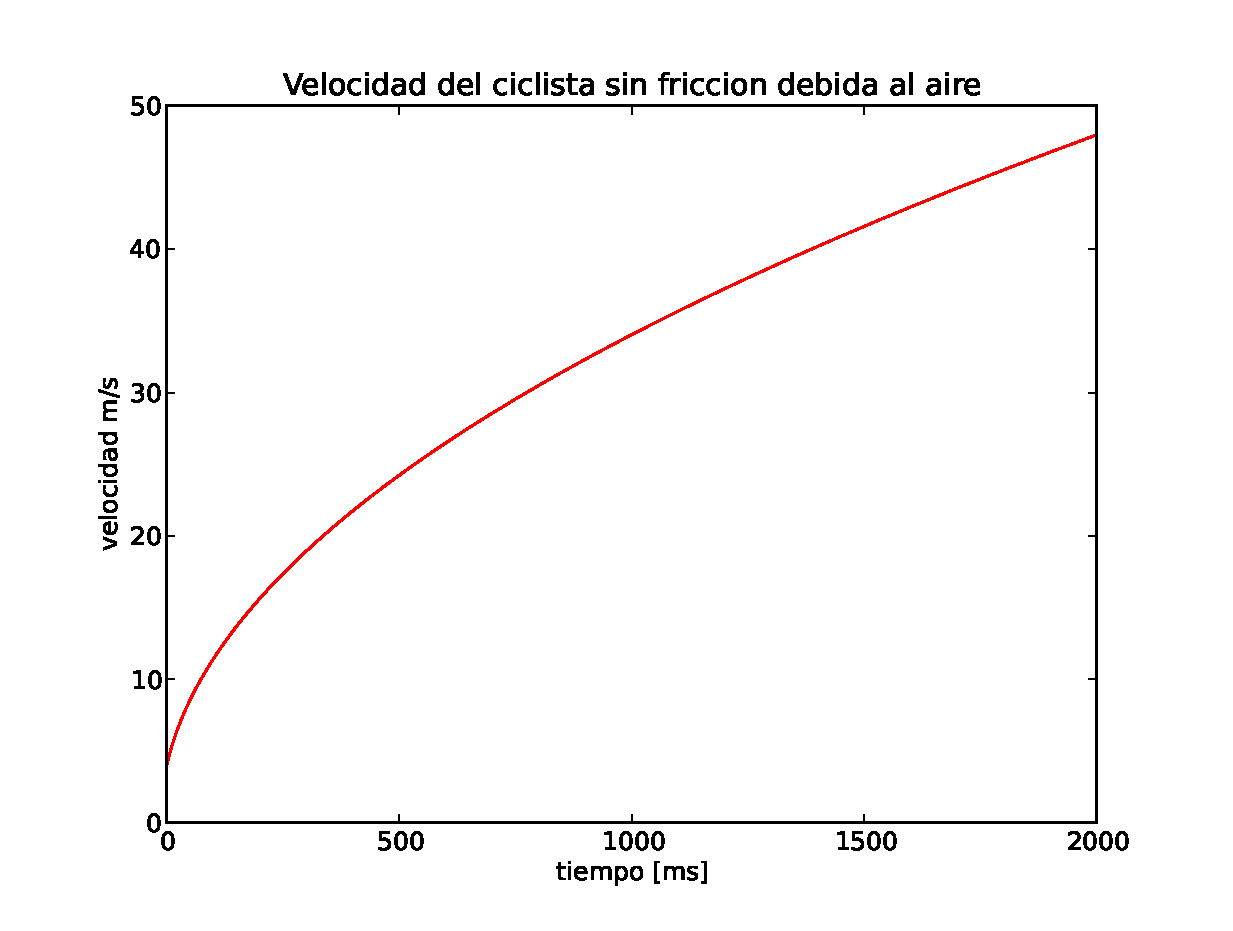
\includegraphics[scale=0.6]{Imagenes/EjerBicicleta01.eps}
\end{figure}
\end{frame}
\begin{frame}
\frametitle{Interpretación de los resultados}
\textbf{¿Es congruente la solución numérica con la física?}
\\
\bigskip
\pause
La solución de la ecuación de movimiento (\ref{EqPotenciavel}) es correcta, pero nuestro trabajo no concluye aquí:
\pause
\begin{alertblock}{La física no checa}
La solución predice que la velocidad del ciclista se incrementará sin límite para tiempos muy largos.
\end{alertblock}
\end{frame}
\begin{frame}
\frametitle{Ajuste en el modelo inicial}
Vamos a corregir este resultado: cuando se generaliza el modelo se debe de incluir el efecto de la resistencia del aire.
\\
\bigskip
\pause
El nuevo término que vamos a añadir a la ecuación de movimiento nos obliga a desarrollar una solución numérica, así que con eso en mente se considera un tratamiento numérico de la ec. (\ref{EqPotenciavel})
\end{frame}
\begin{frame}
\frametitle{Abordaje numérico}
Comenzamos con la forma de diferencias finitas para la derivada de la velocidad
\begin{align}
\dv{v}{t} \simeq \dfrac{v_{i+1} - v_{i}}{\Delta t}
\label{Eqderivada}
\end{align}
donde asumimos que $\Delta t$ es paso discreto pequeño, y $v_{i}$ es la velocidad al tiempo $t_{i} \equiv i \Delta t$.
\end{frame}
\begin{frame}
\frametitle{Abordaje numérico}
Por lo que de la ecuación (\ref{EqPotenciavel}), tenemos que la velocidad al paso $i+1$ es:
\begin{align}
v_{i+1} = v_{i} + \dfrac{P}{m \, v_{i}} \Delta t
\label{Eqveli+1}
\end{align}
\end{frame}
\begin{frame}
\frametitle{Calculando la velocidad}
Dada la velocidad en un tiempo $i$ (es decir, $v_{i}$), podemos usar la ec. (\ref{Eqveli+1}), para calcular un valor \textit{aproximado} de la velocidad en el siguiente paso $v_{i+1}$.
\end{frame}
\begin{frame}
\frametitle{Calculando la velocidad}
Si conocemos la velocidad inicial $v_{0}$, podemos obtener $v_{1}$, $v_{2}$, y así sucecivamente.
\\
\bigskip
Ahora hay que introducir en la ecuación, los parámetros de fricción debida al aire.
\end{frame}
\begin{frame}
\frametitle{Considerando la fricción del aire}
La fuerza debida a la fricción puede aproximarse de manera inicial como
\begin{align}
F_{a} \simeq - B_{1} \: v - B_{2} \: v^{2}
\label{EqFfriccion}
\end{align}
\end{frame}
\begin{frame}
\frametitle{Considerando la fricción del aire}
\begin{align*}
F_{a} \simeq - B_{1} \: v - B_{2} \: v^{2}
\end{align*}
Para velocidades muy bajas, el primer término es el que domina, y su coeficiente $B_{1}$ se puede calcular para objetos con formas sencillas.
\end{frame}
\begin{frame}
\frametitle{Considerando la fricción del aire}
\begin{align*}
F_{a} \simeq - B_{1} \: v - B_{2} \: v^{2}
\end{align*}
Para una velocidad razonable $v^{2}$ el término domina sobre los demás, pero el coeficiente $B_{2}$ no puede calcularse exactamente en objetos sencillos como una pelota de beisbol, menos para una bicicleta.
\end{frame}
\begin{frame}
\frametitle{Primera aproximación}
Podemos aproximar el valor de $B_{2}$ como sigue:
\\
\medskip
\pause
Si un objeto se mueve a través de la atmósfera, entonces debe empujar al aire delante fuera del camino.
\end{frame}
\begin{frame}
\frametitle{Primera aproximación}
La masa de aire movido en el tiempo $\dd{t}$ es
\begin{align*}
m_{\text{\tiny{aire}}} \sim \rho \: A \: v \: \dd{t}
\end{align*}
donde $\rho$ es la densidad del aire y $A$ el área frontal del objeto. 
\\
\bigskip
\pause
A este aire se le da una velocidad de orden $v$, y por lo tanto, su energía cinética es
\begin{align*}
E_{\text{\tiny{aire}}} \sim m_{\text{\tiny{aire}}} \: v^{2} /2
\end{align*}
\end{frame}
\begin{frame}
\frametitle{Primera aproximación}
Este es también el trabajo realizado por la fuerza de arrastre (la fuerza sobre el objeto debido a la resistencia del aire) en el tiempo $\dd{t}$, por lo que
\begin{align*}
F_{a} \: v \: \dd{t} = E_{\text{\tiny{aire}}}
\end{align*}
\bigskip
\pause
Poniendo todo esto junto nos encontramos con:
\begin{align*}
F_{a} \simeq - C \: \rho \: A \: v^{2}
\end{align*}
\end{frame}
\begin{frame}
\frametitle{Coeficiente de arrastre}
De la expresión
\begin{align*}
F_{a} \simeq - C \: \rho \: A \: v^{2}
\end{align*}
Tenemos que $C$ es el coeficiente de arrastre, podemos argumentar que tiene un valor de $0.5$ (¿cómo lo demostrarías?).
\end{frame}
\begin{frame}
\frametitle{Coeficiente de arrastre}
Recordemos que estamos haciendo una primera aproximación, si nos interesa contar con una expresión que determine la correcta relación de $F_{a}$ con $v$ y $A$, entonces tendremos que hacer mediciones en un túnel de viento, para utilizar el valor correcto de $C$.
\end{frame}
\begin{frame}
\frametitle{Nueva expresión para la velocidad}
Incluyendo este término en la expresión para la velocidad
\begin{align}
v_{i+1} = v_{i} + \dfrac{P}{m v_{i}} \Delta t - \dfrac{C \rho A v_{i}^{2}}{m} \Delta t
\label{Eqvelifriccion}
\end{align}
Considera los siguientes valores:
\setbeamercolor{item projected}{bg=green!70!black,fg=white}
\setbeamertemplate{enumerate items}[circle]
\begin{enumerate}[<+->]
\item Coeficiente de arrastre: $C = 0.5$
\item Sección de área frontal: $0.33 \: \si{\square\meter}$
\item Masa del sistema ciclista-bicicleta: $70 \: \si{\kilogram}$
\item Velocidad inicial: $4 \: \si{\meter\per\second}$
\item Incremento en el tiempo: $\Delta \: t = 0.1 \: \si{\second}$
\end{enumerate}
\end{frame}
\begin{frame}[allowframebreaks, fragile]
\frametitle{Agregando código}
Agrega lo siguiente en tu código, te recomendamos guardar con otro nombre tu archivo.
\begin{lstlisting}[style=codigopython]
vA_2_B = []

A, C = 0.33, 0.5

#dentro del ciclo for
vc = vA_2_B[i-A_1_B] + potencia*dt / (masa* vA_2_B[i-A_1_B]) - (C*A*vA_2_B[i-A_1_B] ** 2) * dt/masa
    
vA_2_B.append(vc)

#en la graficacion cambia
plt.plot(v, "r-", label="Sin friccion")

#agrega lo siguiente
plt.plot(vA_2_B, "b-", label="Velocidad con friccion")
plt.legend(loc="upper left")

plt.title("Comparacion de la velocidad del ciclista")
plt.axis([0, 210, 0, 50])

plt.show()
\end{lstlisting}
\end{frame}
\begin{frame}
\frametitle{Comparando velocidades}
\begin{figure}
	\centering
	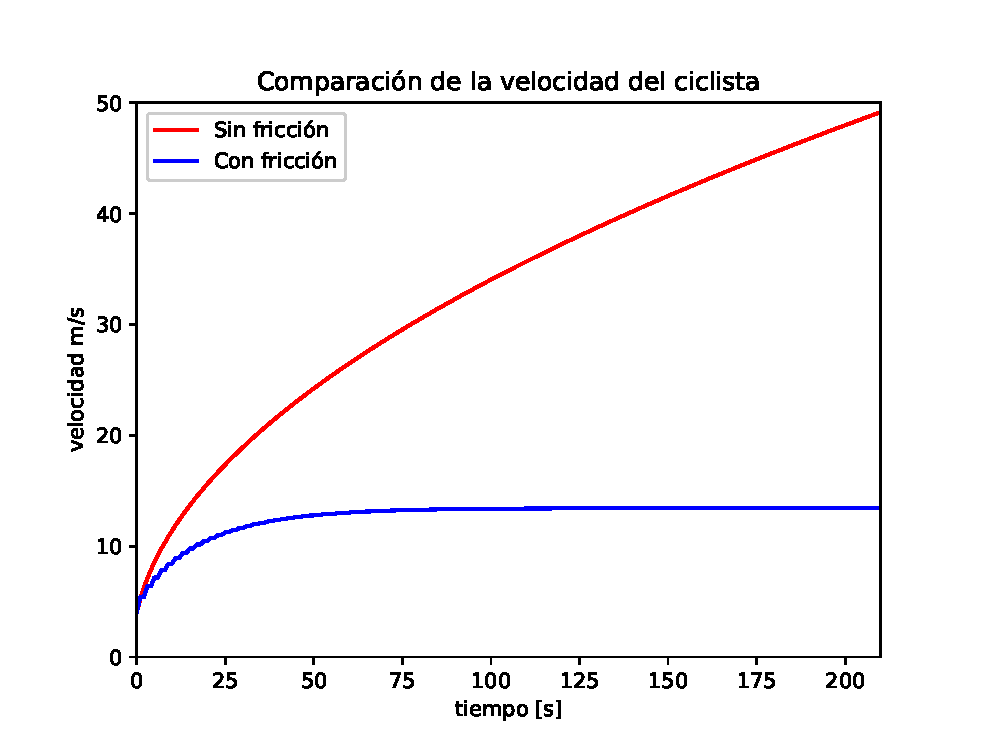
\includegraphics[scale=0.6]{Imagenes/EjerBicicleta02.eps}
\end{figure}
\end{frame}
\begin{frame}
\frametitle{Conclusión}
Con este ejercicio encontramos que no necesariamente una solución que funcione desde el punto de vista informático, tendrá consistencia con la física.
\\
\bigskip
Será nuestra tarea verificar que esa congruencia se mantenga en nuestros algoritmos y soluciones.
\end{frame}
\end{document}